\part{Barcodes}
\ppartpage[\insertpart]{von Sebastian Muszytowski}

%\section{Willkommen!}
%\begin{frame}{Herzlich Willkommen}
%	 \hfill{}\includegraphics[width=0.75\textwidth]{muzy/hello_world_crop.png}\hfill\hbox{}
%\end{frame}

\section{Was ist ein Barcode?}
\begin{frame}[<+->]{Was ist ein Barcode?}
	\begin{itemize}
	\pause
	\item Graphischer Datenspeicher
	\item Mögliche Datentypen (Nicht jeder Barcodetyp kann alles codieren):
		\begin{itemize}
		\item Zahlen (0-9)
		\item Buchstaben (a-z,A-Z)
		\item Alphanumerische Zeichen (a-z,A-Z,0-9)
		\item ASCII
		\item Kodierte Binärdaten (Base64)
		\item Binärdaten
		\end{itemize}
	\end{itemize}
\end{frame}

\section{Barcodetypen}

\begin{frame}[<+->]{Barcodetypen}
	\begin{itemize}
	\item 1D-Codes: Strichmuster (Barcode)
	\item 2D-Codes: Matrix
	\item 3D-Codes: Matrix mit Farben
	\item 4D-Codes: Matrix mit Farben und Zeitachse
	\item Hybride Barcodes: Mischungen zwischen Barcodetypen (z.B. 1D und 2D)
	\end{itemize}
\end{frame}

\subsection{Vergleich der Code-Typen}
\begin{frame}{Vergleich der Code-Typen}
	\hfill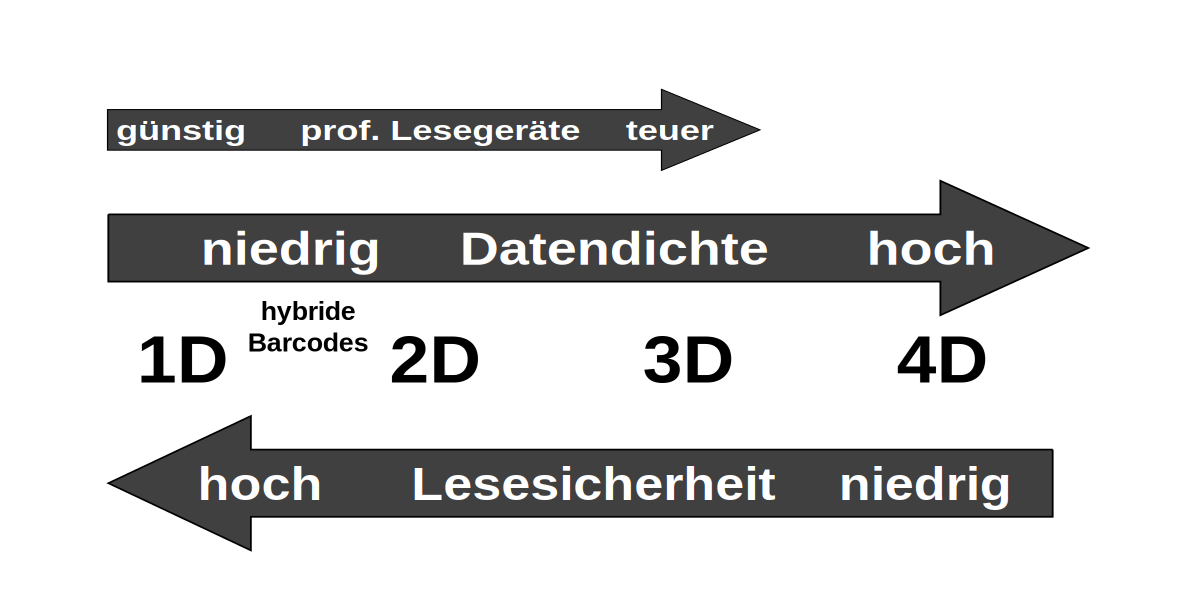
\includegraphics[width=.95\textwidth]{muzy/vergleich.pdf}\hfill\hbox{}
\end{frame}

\section{1D-Codes}

\subsection{Handelsstrichcodes}

\begin{frame}{1D-Codes: Handelsstrichcodes}
	\begin{columns}
	\column{.65\textwidth}
		\begin{itemize}
		\item Beispiel: EAN (European Article Number)
		\item Erlaubte Zeichen: 0-9
		\item Auf fast jedem Produkt zu finden
		\item Prüfziffer ist vorhanden
		\end{itemize}
	\column{.35\textwidth}
		\includegraphics[width=\textwidth]{muzy/1d-ean.pdf}
	\end{columns}
\end{frame}


\section{2D-Codes}

\begin{frame}{2D-Barcodes}
	\onslide*<1>{\includegraphics[width=\textwidth]{muzy/2d-overview-woborder.png}}
	\onslide*<2>{\includegraphics[width=\textwidth]{muzy/2d-overview-controlchars.png}}
	\onslide+<2>{\\\hfill{}Steuerzeichen rot markiert\hfill\hbox{}}
\end{frame}

\subsection{Vor- und Nachteile}
\begin{frame}{2D-Codes: Vor- und Nachteile}
	\begin{itemize}
	\item Vorteile
		\begin{itemize}
		\item Hohe Datendichte
		\item Fehlertoleranzen bis 30\%
		\item Je nach Software hohe Lesesicherheit
		\end{itemize}
	\item Nachteile
		\begin{itemize}
		\item Je nach Software
			\begin{itemize}
			\item Schlechte Lesesicherheit bei leicht gedrehten oder verzerrten Codes
			\item Langsame Lesegeschwindigkeit
			\end{itemize}
		\item Lesegeräte vergleichsweise aufwendig
		\end{itemize}
	\end{itemize}
\end{frame}

\section{3D-Codes}

\begin{frame}{3D-Codes}
	\begin{columns}
	\column{.65\textwidth}
		\begin{itemize}
		\item 2D-Codes mit zusätzlicher Dimension
		\item Dritte Dimension ist meist Farbe
		\item Beispiel: High Capacity Color Barcode (Microsoft)
		\end{itemize}
	\column{.35\textwidth}
		\includegraphics[width=\textwidth]{muzy/3d-hccb.pdf}
	\end{columns}
\end{frame}

\subsection{Vor- und Nachteile}
\begin{frame}{3D-Codes: Vor- und Nachteile}
	\begin{itemize}
	\item Vorteile
		\begin{itemize}
		\item Höhere Datendichte als 2D-Codes
		\end{itemize}
	\item Nachteile
		\begin{itemize}
		\item Noch keine Nutzung
		\item Weitestgehend unbekannt
		\item Alle Nachteile von 2D-Codes
		\item Lesegeräte noch komplizierter und störungsanfälliger
		\end{itemize}
	\end{itemize}
\end{frame}

\section{4D-Codes}

\begin{frame}{4D-Codes}
	\begin{columns}
	\column{.65\textwidth}
		\begin{itemize}
		\item 3D-Codes mit zusätzlicher Dimension
		\item Vierte Dimension ist Zeit
		\end{itemize}
	\column{.35\textwidth}
		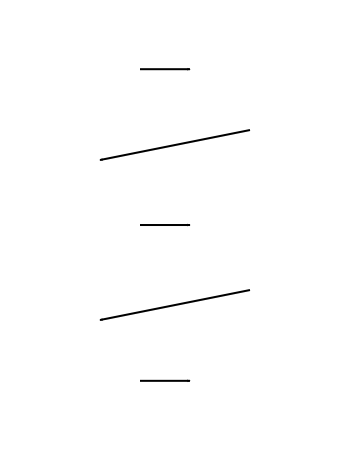
\includegraphics[width=\textwidth]{muzy/4d-concept.pdf}
	\end{columns}
\end{frame}

\subsection{Vor- und Nachteile}
\begin{frame}{4D-Codes: Vor- und Nachteile}
	\begin{itemize}
	\item Vorteile
		\begin{itemize}
		\item Noch höhere Datendichte
		\end{itemize}
	\item Nachteile
		\begin{itemize}
		\item Noch fehleranfälliger durch das Filmen des Barcodes
		\item Alle Nachteile von 3D-Codes
		\end{itemize}
	\end{itemize}
\end{frame}

\begin{frame}{Hybride Barcodes}
	\begin{columns}
	\column{.65\textwidth}
		\begin{itemize}
		\item Mischung aus 1D Barcodes und 2D Matrixcodes
		\item Bekanntester Vertreter PDF417
		\end{itemize}
	\column{.35\textwidth}
		\includegraphics[width=\textwidth]{muzy/pdf417.png}
	\end{columns}
\end{frame}

\subsection{Vor- und Nachteile}
\begin{frame}{Hybride Barcodes: Vor- und Nachteile}
	\begin{itemize}
	\item Vorteile
		\begin{itemize}
		\item Höhere Datendichte als 1D Barcodes
		\item Fehlerkorrekturverfahren vorhanden
		\item Kann mit 1D Barcodescannern gelesen werden
		\end{itemize}
	\item Nachteile
		\begin{itemize}
		\item Wird von 2D Matrixcodes verdrängt 
		\end{itemize}
	\end{itemize}
\end{frame}


\section{Dekodieren von Barcodes}
\begin{frame}{Dekodieren von Barcodes am Beispiel: Code128}
	\pause
	\begin{columns}
	\column{.65\textwidth}
		\begin{itemize}
		\item Erlaubte Zeichen: ASCII
		\item Drei verschiedene Subcodes, für effizientere Kodierung von bestimmtem Input
		\item Möglichkeit zwischen Subcodes zu wechseln
		\end{itemize}
	\column{.35\textwidth}
		\includegraphics[width=\textwidth]{muzy/1d-128.pdf}
	\end{columns}
\end{frame}

\subsection{weitere Merkmale}
\begin{frame}{Weitere Merkmale von Code128}
	\begin{itemize}
	\item Es gibt START und STOP Zeichen
	\item Jedes Zeichen ist mit 11 Strichen codiert
	\item Nur das STOP Zeichen ist mit 13 Strichen codiert
	\item Es gibt eine Prüfsumme
	\end{itemize}
\end{frame}

\subsection{Dekodieren eines Barcodes}
\begin{frame}{Ein Code128}
	\hfill\includegraphics[width=.95\textwidth]{muzy/cake_1.png}\hfill\hbox{}
\end{frame}

\begin{frame}{Ein Code128 - Strichbreiten}
	\hfill\includegraphics[width=.95\textwidth]{muzy/cake_2.png}\hfill\hbox{}
\end{frame}

\begin{frame}{Ein Code128 - Strichbreiten im Detail}
	\hfill\includegraphics[width=.95\textwidth]{muzy/cake_4.png}\hfill\hbox{}
\end{frame}

\begin{frame}{Ein Code128 - Strichbreiten im Detail}
	\hfill\includegraphics[width=.95\textwidth]{muzy/cake_5.png}\hfill\hbox{}
	\hfill Jedes Zeichen ist 11 Striche breit (STOP-Zeichen 13) \hfill\hbox{}
\end{frame}

\begin{frame}{Ein Code128 - Die Segmente im Detail}
	\hfill\includegraphics[width=.95\textwidth]{muzy/cake_6.png}\hfill\hbox{}
\end{frame}

\begin{frame}{Ein Code128 - Die Segmente im Detail}
	\hfill Nun das Dekodiersheet zur Hand nehmen! \hfill\hbox{}
\end{frame}

\begin{frame}{Ein Code128 - Erfassen der Balken und Leerzeichen Breite}
	\hfill\includegraphics[width=.95\textwidth]{muzy/cake_7.png}\hfill\hbox{}
\end{frame}

\begin{frame}{Ein Code128 - Dekodieren}
	\hfill\includegraphics[width=.95\textwidth]{muzy/cake_8.png}\hfill\hbox{}
	\hfill Mithilfe des Dekodiersheets kann nun jedes Zeichen dekodiert werden. \hfill\hbox{}
\end{frame}
\begin{frame}{Ein Code128 - Dekodieren}
	\hfill\includegraphics[width=.95\textwidth]{muzy/cake_8.png}\hfill\hbox{}
	\hfill Es lassen sich Steuerzeichen, Nutzdaten sowie eine Prüfsumme erkennen. \hfill\hbox{}
\end{frame}

\begin{frame}{Ein Code128 - Erfassen der Daten}
	\hfill\includegraphics[width=.95\textwidth]{muzy/cake_9.png}\hfill\hbox{}
\end{frame}

\begin{frame}{Ein Code128 - Erfassen der Daten}
	\hfill
\includegraphics[width=.35\textwidth]{muzy/cake.png}\hfill\hbox{}
	\hfill CAKE! \hfill\hbox{}
\end{frame}

\begin{frame}{Berechnung der Prüfsumme}
	\begin{itemize}
	\item Ziel: Prüfung der Daten auf Korrektheit
	\item Berechnung: 
	\item 1x Startz. + 1x 1. Wert + 2x 2. Wert [...]
	\item Summe div 103, Rest = Prüfsumme	
	\end{itemize}
\end{frame}

\begin{frame}{Berechnung der Prüfsumme}
	\begin{itemize}
	\item In unserem Beispiel:
	\item 104 (StartB) + 1x 67 (c) + 2x 65 (a) + 3x 75 (k) + 4x 69 (e)
	\item =802 | 802 mod 103 = 81 = Prüfzeichen "q"
	\end{itemize}
\end{frame}

\section{Lösung des Tasksheets}
\begin {frame}[<+->]{Lösung des Tasksheets}
	\begin{itemize}
	\item Sheet 01: \texttt{A\textvisiblespace{}place\textvisiblespace{}}
	\item Sheet 02: \texttt{and\textvisiblespace{}a\textvisiblespace{}ti}
	\item Sheet 03: \texttt{me,\textvisiblespace{}neit}
	\item Sheet 04: \texttt{her\textvisiblespace{}one\textvisiblespace{}}
	\item Sheet 05: \texttt{too\textvisiblespace{}far\textvisiblespace{}}
	\end{itemize}
\end{frame}

\begin {frame}[<+->]{Lösung des Tasksheets}
	\begin{itemize}
	\item Sheet 06: \texttt{away.\textvisiblespace{}51}
	\item Sheet 07: \texttt{.2139\textvisiblespace{}6.}
	\item Sheet 08: \texttt{7845\textvisiblespace{}201}
	\item Sheet 09: \texttt{0-08-07\textvisiblespace{}}
	\item Sheet 10: \texttt{18:00:00}
	\end{itemize}
\end{frame}

\begin{frame}{A place and a time, neither one too far away.}
	\hfill 51.2139 6.7845 2010-08-07 18:00:00 \hfill\hbox{}
\end{frame}
